\scanpage{72}
% archive sheet number: 71

$\underline{Q}_p$ faisceaux constructibles sur $k$ vers la catégorie $\mathrm{Fcriso}(k)$. Pour un objet \deleted{$E$}$(E,F_E)$ de cette dernière, les conditions suivantes sont équivalentes\inserted{\unsure{\deleted{x}(|\deleted{(}x}si $k$ parfait\unsure{\deleted{x})|\deleted{)}x}}\handwritten{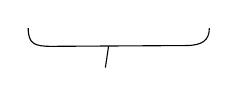
\begin{tikzpicture}[x=1cm,y=1cm,baseline=0cm]\draw[thin] (0,.2)..controls (0,0) and (.08,-.03)..(.3,-.03)--(2,-.02)..controls (2.2,-.02) and (2.3,.04)..(2.3,.2);\draw[thin] (1.02,-.03)--(.98,-.3);\end{tikzpicture}}: a) $(E,F_E)$ appartient à l'image essentielle du foncteur précédent; b) il existe un réseau $M\subset E$ stable par $F_E$ \deleted{sur} \uline{\unsure{\deleted{l}e|\deleted{e}l}t} par $F_E^{-1}$ (i.e. tel que $F_E$ induise un \uline{automorphisme} de $M$); c) la famille des i\unsure{\handwritten{t}|\deleted{e}\handwritten{t}|\deleted{o}\handwritten{t}|\deleted{a}\handwritten{t}}érés $F^{\unsure{n|m}}$, $n\quad\underline{Z}$, est bornée ; d) $E$ et $\overset{\handwritten{\vee}}{E}$ sont effectifs.

Les F-isocristaux en question sont appelés ``trivaux'' ou ``\uline{de pente nulle}''. On trouve ainsi un \uline{épimorphisme de gerbes}
\figure{\[
\underline{G}(k)\handwritten{\longrightarrow}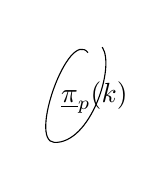
\begin{tikzpicture}[baseline=(gerbe.base)]
\node[inner sep=1pt] (gerbe) {$\handwritten{\underline{\pi}_{p}}(k)$};
\handwritten{\draw[thin] (-0.08,0.57) .. controls (-0.33,0.88) and (-0.84,-0.55) .. (-0.51,-0.57) .. controls (-0.05,-0.59) and (0.27,0.39) .. (0.10,0.64);}
\end{tikzpicture}\ ,
\]}
\margin{\handwritten{$\Pi$\par majuscule?}}
où $\handwritten{\underline{\unsure{\Pi|\pi}}}_p(k)$ est la gerbe sur $\underline{Q}_p$ \deleted{des représentations continues} associée à la catégorie tannakienne des $\underline{Q}_p$-faisceaux constructibles, équivalente \deleted{à l'enveloppe alg} (une fois choisie une clôture algébrique $\bar{k}$ de $k$) à la gerbe triviale définie par l'enveloppe algébrique \deleted{du} $p$-adique du groupe pro-fini $\handwritten{\pi}=\operatorname{Gal}(\handwritten{\bar{k}}/k)$. Tenant compte de l'homomorphisme d'augmentation de \unsure{\deleted{T}G|\deleted{G}T}ate, on trouve même un homomorphisme
\[
\underline{G}(k)\handwritten{\longrightarrow\underline{\pi}}_p(k)\ \mathrm{x}\ \handwritten{[}\underline{G}_m\handwritten{]}_{\underline{Q}_p}
\]
où $\handwritten{[}\underline{G}_m\handwritten{]}$ est la gerbe triviale définie par $\underline{G}_m$ . On vérifie facilement que c'est encore un épimorphisme (i.e. que le foncteur
\[
(V_i)_{\handwritten{i}}\handwritten{\longmapsto\sum}V_i\otimes_{\underline{\unsure{\not Q|\mathbb{Q}}}_p}\underline{Q}_p(i)
\]
allant de la catégorie des \deleted{\unsure{sh|ch}} $\underline{Q}_p$-faisceaux constructibles \inserted{\handwritten{gradu\unsure{i|é}s}}\handwritten{\begin{tikzpicture}[x=1cm,y=1cm,baseline=0cm]\draw[thin] (0,-.35)..controls (.12,-.15) and (-.05,.1)..(.4,.25)..controls (1.2,.4) and (2.25,.7)..(2.5,.92)..controls (2.65,1.1) and (2.55,1.22)..(2.4,1.2);\end{tikzpicture}} sur $k$ vers $\mathrm{Fcriso}(k)$ est pleinement fidèle). Les F-isocristaux de la forme précédente pourraient être appelés les F-isocristaux \uline{de niveau zéro} .

\handwritten{6.} Considérons maintenant un homomor\unsure{\^{p}|\deleted{ô}p|\deleted{p}ô}\unsure{\.{h}|\deleted{i}h|\deleted{h}i}isme de corps\textsubscript{\unsure{x|\deleted{x}}}
\[
k\handwritten{\longrightarrow}k'\ ,
\]
d'où un homomorphisme de catégories tannakiennes sur $\underline{Q}_p$
\[
\mathrm{Fcriso}(k)\handwritten{\longrightarrow}\mathrm{Fcriso}(\deleted{\unsure{i|t|k}}\handwritten{k}')\ ,
\]
et un homomorphisme de gerbes tannakiennes sur $\underline{Q}_p$ en sens inverse

\mspage{71}
